\documentclass[border=4pt]{standalone}

\usepackage{amsmath}
\usepackage{tikz}
\usepackage{mathdots}
\usepackage{yhmath}
\usepackage{cancel}
\usepackage{color}
\usepackage{siunitx}
\usepackage{array}
\usepackage{multirow}
\usepackage{amssymb}
\usepackage{gensymb}
\usepackage{tabularx}
\usepackage{booktabs}
\usetikzlibrary{fadings}
\usetikzlibrary{patterns}


\begin{document}
 
 

\tikzset{every picture/.style={line width=0.75pt}} %set default line width to 0.75pt        

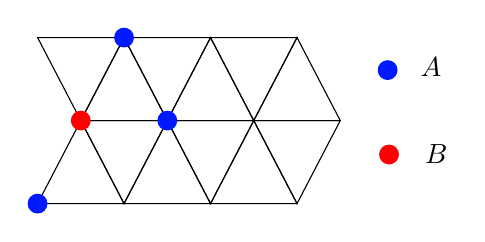
\begin{tikzpicture}[x=0.75pt,y=0.75pt,yscale=-1,xscale=1]
%uncomment if require: \path (0,493); %set diagram left start at 0, and has height of 493

%Shape: Triangle [id:dp09273907309237184] 
\draw   (190.83,90.33) -- (211.67,130.33) -- (170,130.33) -- cycle ;
%Shape: Triangle [id:dp43742707176740714] 
\draw   (232.5,90.33) -- (253.33,130.33) -- (211.67,130.33) -- cycle ;
%Shape: Triangle [id:dp17022653848603597] 
\draw   (274.17,90.33) -- (295,130.33) -- (253.33,130.33) -- cycle ;
%Shape: Triangle [id:dp7393478132297682] 
\draw   (190.83,170.33) -- (170,130.33) -- (211.67,130.33) -- cycle ;
%Shape: Triangle [id:dp11132914728548027] 
\draw   (232.5,170.33) -- (211.67,130.33) -- (253.33,130.33) -- cycle ;
%Shape: Triangle [id:dp041317246113506956] 
\draw   (274.17,170.33) -- (253.33,130.33) -- (295,130.33) -- cycle ;
%Shape: Triangle [id:dp8410625900438737] 
\draw   (211.67,130.33) -- (190.83,90.33) -- (232.5,90.33) -- cycle ;
%Shape: Triangle [id:dp18440550097115738] 
\draw   (253.33,130.33) -- (232.5,90.33) -- (274.17,90.33) -- cycle ;
%Shape: Triangle [id:dp7818432388110512] 
\draw   (211.67,130.33) -- (232.5,170.33) -- (190.83,170.33) -- cycle ;
%Shape: Triangle [id:dp3667265901710903] 
\draw   (253.33,130.33) -- (274.17,170.33) -- (232.5,170.33) -- cycle ;
%Shape: Triangle [id:dp7478479851644764] 
\draw   (170,130.33) -- (149.17,90.33) -- (190.83,90.33) -- cycle ;
%Shape: Triangle [id:dp30189854422644635] 
\draw   (170,130.33) -- (190.83,170.33) -- (149.17,170.33) -- cycle ;
%Shape: Circle [id:dp1477225677089331] 
\draw  [color={rgb, 255:red, 0; green, 25; blue, 255 }  ,draw opacity=1 ][fill={rgb, 255:red, 0; green, 25; blue, 255 }  ,fill opacity=1 ] (144.67,170.33) .. controls (144.67,167.85) and (146.68,165.83) .. (149.17,165.83) .. controls (151.65,165.83) and (153.67,167.85) .. (153.67,170.33) .. controls (153.67,172.82) and (151.65,174.83) .. (149.17,174.83) .. controls (146.68,174.83) and (144.67,172.82) .. (144.67,170.33) -- cycle ;
%Shape: Circle [id:dp6341954229843652] 
\draw  [color={rgb, 255:red, 0; green, 25; blue, 255 }  ,draw opacity=1 ][fill={rgb, 255:red, 0; green, 25; blue, 255 }  ,fill opacity=1 ] (186.33,90.33) .. controls (186.33,87.85) and (188.35,85.83) .. (190.83,85.83) .. controls (193.32,85.83) and (195.33,87.85) .. (195.33,90.33) .. controls (195.33,92.82) and (193.32,94.83) .. (190.83,94.83) .. controls (188.35,94.83) and (186.33,92.82) .. (186.33,90.33) -- cycle ;
%Shape: Circle [id:dp014741882861695421] 
\draw  [color={rgb, 255:red, 255; green, 0; blue, 0 }  ,draw opacity=1 ][fill={rgb, 255:red, 255; green, 0; blue, 0 }  ,fill opacity=1 ] (165.5,130.33) .. controls (165.5,127.85) and (167.51,125.83) .. (170,125.83) .. controls (172.49,125.83) and (174.5,127.85) .. (174.5,130.33) .. controls (174.5,132.82) and (172.49,134.83) .. (170,134.83) .. controls (167.51,134.83) and (165.5,132.82) .. (165.5,130.33) -- cycle ;
%Shape: Circle [id:dp8712946371764263] 
\draw  [color={rgb, 255:red, 0; green, 25; blue, 255 }  ,draw opacity=1 ][fill={rgb, 255:red, 0; green, 25; blue, 255 }  ,fill opacity=1 ] (207.17,130.33) .. controls (207.17,127.85) and (209.18,125.83) .. (211.67,125.83) .. controls (214.15,125.83) and (216.17,127.85) .. (216.17,130.33) .. controls (216.17,132.82) and (214.15,134.83) .. (211.67,134.83) .. controls (209.18,134.83) and (207.17,132.82) .. (207.17,130.33) -- cycle ;
%Shape: Circle [id:dp060018492159648495] 
\draw  [color={rgb, 255:red, 0; green, 25; blue, 255 }  ,draw opacity=1 ][fill={rgb, 255:red, 0; green, 25; blue, 255 }  ,fill opacity=1 ] (313.33,106) .. controls (313.33,103.51) and (315.35,101.5) .. (317.83,101.5) .. controls (320.32,101.5) and (322.33,103.51) .. (322.33,106) .. controls (322.33,108.49) and (320.32,110.5) .. (317.83,110.5) .. controls (315.35,110.5) and (313.33,108.49) .. (313.33,106) -- cycle ;
%Shape: Circle [id:dp1245110266249636] 
\draw  [color={rgb, 255:red, 255; green, 0; blue, 0 }  ,draw opacity=1 ][fill={rgb, 255:red, 255; green, 0; blue, 0 }  ,fill opacity=1 ] (314,146.67) .. controls (314,144.18) and (316.01,142.17) .. (318.5,142.17) .. controls (320.99,142.17) and (323,144.18) .. (323,146.67) .. controls (323,149.15) and (320.99,151.17) .. (318.5,151.17) .. controls (316.01,151.17) and (314,149.15) .. (314,146.67) -- cycle ;

% Text Node
\draw (338.67,104.33) node   {$A$};
% Text Node
\draw (341.33,146.33) node   {$B$};


\end{tikzpicture}


\end{document}
